\documentclass[12pt,a4paper]{article}
\usepackage[margin=2.2cm]{geometry}
\usepackage{enumitem}
\usepackage{titlesec}
\usepackage{hyperref}
\usepackage{xcolor}
\usepackage{booktabs}
\usepackage{parskip}
\usepackage{amsmath}
\usepackage{graphicx}
\usepackage{float}
\usepackage{tcolorbox}
\tcbuselibrary{breakable,skins}

\definecolor{accent}{RGB}{30,70,120}
\definecolor{green}{RGB}{40,120,40}
\definecolor{red}{RGB}{180,40,40}
\definecolor{strongbg}{RGB}{230,245,230}
\definecolor{strongframe}{RGB}{60,140,60}
\definecolor{warnbg}{RGB}{255,250,230}
\definecolor{warnframe}{RGB}{180,150,40}
\definecolor{failbg}{RGB}{255,235,235}
\definecolor{failframe}{RGB}{180,60,60}

\newtcolorbox{kbox}[2][]{
    enhanced, colback=#2bg, colframe=#2frame,
    boxrule=1pt, arc=3pt, left=8pt, right=8pt, top=6pt, bottom=6pt,
    fonttitle=\bfseries\large, coltitle=white, title={#1}, breakable,
}

\titleformat{\section}{\Large\bfseries\color{accent}}{}{0em}{}[\titlerule]
\setlength{\parskip}{0.6em}
\hypersetup{colorlinks=true, linkcolor=accent, urlcolor=accent}

\begin{document}

\begin{center}
\vspace*{0.5cm}
{\Huge\bfseries\color{accent} Concepts}\\[0.8em]
{\Large Copper · Gas · Bitcoin · Sol}\\[1.5em]
{\small Robin Langer · August 2026}
\end{center}

\vspace{0.8em}

\begin{kbox}[Start here: what we are doing]{strong}
A rule looks at trading activity once a day and says \textbf{hold} or
\textbf{cash} for each of four things: copper, natural gas, Bitcoin,
and Solana.

\vspace{0.7em}
One pot of money serves all four. When one says ``sit out,'' the money
goes where another says ``get in.''

\vspace{0.7em}
Solana is the wild one --- biggest gains, biggest crashes. We cap it at
a quarter of the pot, deliberately.
\end{kbox}

\section{1. Losing hurts more than winning helps}

\begin{kbox}[The most important fact in this document]{strong}
Lose $50\%$, then gain $50\%$. You are \textbf{not} back to even:
\[
    0.50 \times 1.50 = 0.75 \quad\longrightarrow\quad \text{down } 25\%.
\]

\vspace{0.3em}
To climb out of a hole you need a bigger gain than the loss that made it:

\vspace{0.4em}
\centering
\begin{tabular}{@{}rr@{}}
    \toprule
    \textbf{You lose} & \textbf{You need to get back} \\
    \midrule
    $-25\%$ & $+33\%$ \\
    $-50\%$ & $+100\%$ \\
    $-90\%$ & $+900\%$ \\
    $-96\%$ & $+2{,}400\%$ \\
    \bottomrule
\end{tabular}

\vspace{0.5em}
\raggedright
That last row is real: Solana fell $96\%$ in 2022.

\vspace{0.4em}
\textbf{So: avoiding big losses matters more than catching big gains.}
That is what the whole strategy is for.
\end{kbox}


\newpage
\begin{kbox}[The fair coin that still ruins you]{warn}
Now a game that sounds perfectly fair. Toss a coin. Heads you go
\textbf{up 5\%}, tails you go \textbf{down 5\%}. You win exactly half
the time. Same percentage either way. Surely you break even?

\vspace{0.5em}
No. One win and one loss, in either order:
\[
    1.05 \times 0.95 = 0.9975 \quad\longrightarrow\quad \textbf{down } 0.25\%.
\]

\vspace{0.3em}
Every matched pair of wins and losses quietly costs you a quarter of a
percent. It never stops. Start with \$10{,}000 and keep tossing:

\vspace{0.5em}
\centering
\begin{tabular}{@{}rrr@{}}
    \toprule
    \textbf{Tosses} & \textbf{You have} & \textbf{Change} \\
    \midrule
    10   & \$9{,}876 & $-1.2\%$ \\
    50   & \$9{,}393 & $-6.1\%$ \\
    100  & \$8{,}824 & $-11.8\%$ \\
    200  & \$7{,}786 & $-22.1\%$ \\
    500  & \$5{,}348 & $-46.5\%$ \\
    1000 & \$2{,}861 & $-71.4\%$ \\
    \bottomrule
\end{tabular}

\vspace{0.6em}
\raggedright
\textbf{The trajectory is down. Always down.} Not because you were
unlucky --- you won exactly half your tosses --- but because the $5\%$
you lose is taken off a bigger number than the $5\%$ you win is added
to.

\vspace{0.4em}
To cancel a $5\%$ loss you need $5.26\%$, not $5\%$. That gap is the
whole story, and it compounds.

\vspace{0.5em}
\textbf{This is the enemy.} It has a name --- \emph{volatility drag} ---
and it is why wobble itself costs money, quite apart from being
unpleasant.
\end{kbox}


\begin{figure}[H]
    \centering
    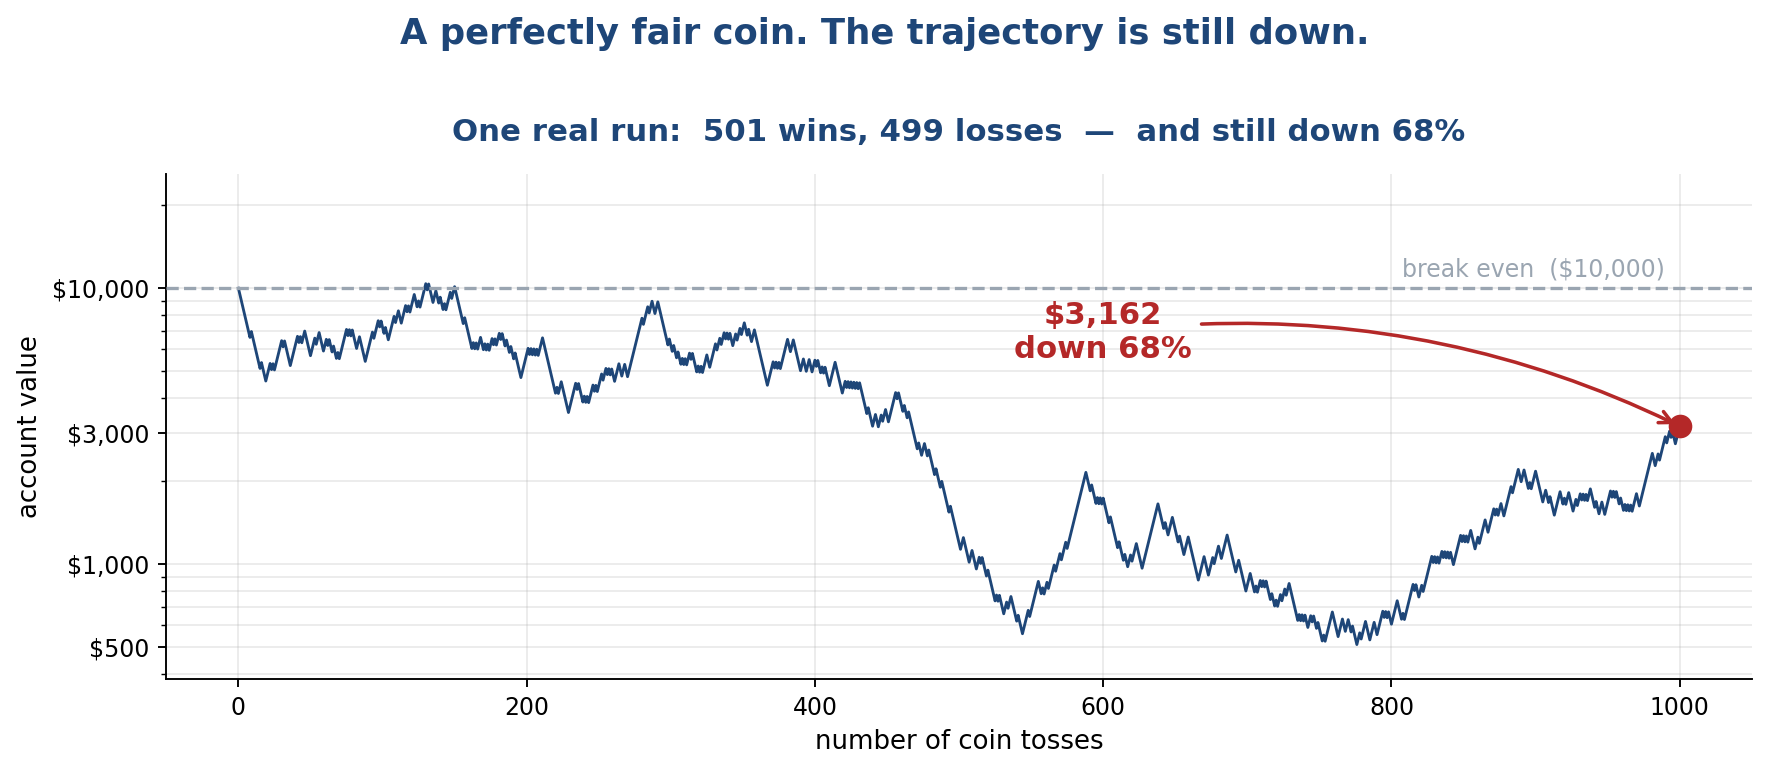
\includegraphics[width=\textwidth]{coin_drag.png}
\end{figure}

\begin{kbox}[What the picture shows]{warn}
One genuine run of 1{,}000 tosses. This coin came up heads \textbf{501}
times and tails 499 --- \emph{more wins than losses} --- and still
finished at \$3{,}162, \textbf{down 68\%}.
\end{kbox}

\begin{kbox}[Being too wobbly is bad]{strong}
\centering
\Large\bfseries
Wobble is not just uncomfortable.\\
Wobble itself loses money.

\vspace{0.7em}
\raggedright\normalsize\normalfont
Two accounts can have identical average returns, and the wobblier one
will end up with less money. Not because of bad luck --- because of the
arithmetic above. The bigger the swings, the worse the bleed:

\vspace{0.5em}
\centering
\begin{tabular}{@{}crl@{}}
    \toprule
    \textbf{Swing size} & \textbf{Cost per win-lose pair} & \\
    \midrule
    $\pm 1\%$  & $-0.01\%$ & barely noticeable \\
    $\pm 5\%$  & $-0.25\%$ & the example above \\
    $\pm 10\%$ & $-1.00\%$ & serious \\
    $\pm 20\%$ & $-4.00\%$ & ruinous \\
    \bottomrule
\end{tabular}

\vspace{0.6em}
\raggedright
Double the wobble and you quadruple the damage.

\end{kbox}

\begin{figure}[H]
    \centering
    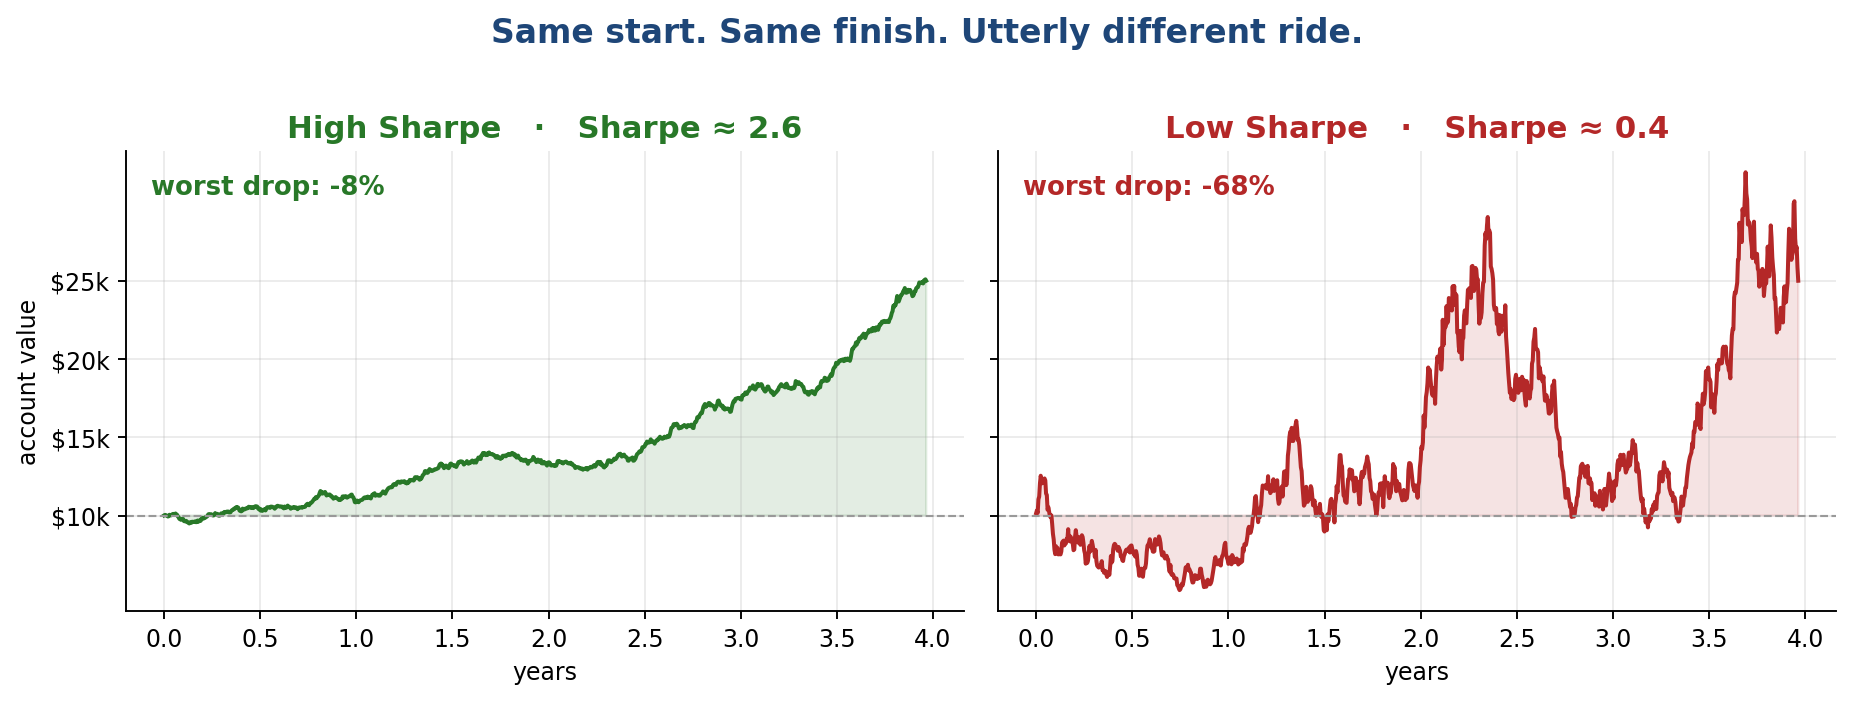
\includegraphics[width=\textwidth]{sharpe_compare.png}
\end{figure}


\section{2. Sharpe --- one number for ``was it worth it?''}

\begin{kbox}[Return alone tells you nothing]{strong}
``I made $150\%$'' is not an achievement until you know what was risked
to get it.

\vspace{0.5em}
So we divide:
\[
    \textbf{Sharpe} = \frac{\text{return}}{\text{wobble}}.
\]

\vspace{0.3em}
\textbf{In words: how much reward you got per unit of stomach-churning
you had to sit through.}

\vspace{0.5em}
All four of our assets score between $0.90$ and $1.34$. The whole
portfolio scores $1.44$.
\end{kbox}

\section{3. Drawdown --- the number that makes people quit}

\begin{kbox}[How deep the holes get]{warn}
``Drawdown'' = the drop from a previous high. Here is the worst drop
for each asset, just holding it, versus holding it only when our rule
says to:

\vspace{0.4em}
\centering
\begin{tabular}{@{}lrr@{}}
    \toprule
    & \textbf{Just holding it} & \textbf{With the rule} \\
    \midrule
    Copper       & $-35\%$ & $-23\%$ \\
    Bitcoin      & $-77\%$ & $-28\%$ \\
    Natural gas  & $-84\%$ & $-53\%$ \\
    Solana       & $-96\%$ & $-79\%$ \\
    \bottomrule
\end{tabular}

\vspace{0.5em}
\raggedright
The rule helps everywhere. It does not make anything safe. Solana is
still the scariest thing on the list \emph{after} the rule has done its
work.
\end{kbox}

\section{4. Don't put all your eggs in one basket}

\begin{kbox}[Why this old saying is mathematically true]{strong}
Our four barely move together. Copper follows Chinese factories,
gas follows the weather, Bitcoin follows its own crowd.

\vspace{0.4em}
When you split money across things that move \emph{independently},
the returns average out but the \textbf{wobble shrinks}:
\[
    \text{wobble} = \frac{\text{wobble of one}}{\sqrt{\text{how many}}}.
\]

\vspace{0.3em}
Four unrelated assets $\Rightarrow$ $\sqrt{4}=2$ $\Rightarrow$
\textbf{half the wobble, same return.} That is as close to a free
lunch as investing gets.

\vspace{0.4em}
And because of idea \#1, less wobble mechanically means \textbf{more
money at the end}, not just a calmer ride.

\vspace{0.4em}
The catch: it only works if the baskets are genuinely
\emph{unrelated}. Owning four things that all crash together is one
bet bought four times.
\end{kbox}

\newpage
\section{5. The rule, in full}

\begin{kbox}[The entire trading rule]{strong}
Each day we combine two things: how much the price moved, and how much
money was traded. Big move on heavy trading counts; the same move on
thin trading barely counts. Add that up over the last 180 days
(90 for gas) and compare it to today's price. Call the answer the
\textbf{ratio}.

\vspace{0.6em}
\begin{center}
\Large
ratio above 1 \;$\longrightarrow$\; \textbf{hold it}\\[0.4em]
ratio 1 or below \;$\longrightarrow$\; \textbf{hold cash}
\end{center}

\vspace{0.5em}
Checked once a day. No borrowing. No betting on things falling. When
the rule says cash, you hold cash and nothing can happen to you.

\vspace{0.4em}
That's it. That's the whole thing.
\end{kbox}

\section{6. One pot, four assets}

\begin{kbox}[Capital recycling]{strong}
Each asset only says ``hold'' about a third to a half of the time. Four
separate accounts would leave most of the money asleep most of the
time. So we use one pot and put it wherever the signals point:

\vspace{0.4em}
\centering
\begin{tabular}{@{}lll@{}}
    \toprule
    \textbf{Signals on} & \textbf{Where the money goes} & \textbf{Cash} \\
    \midrule
    3 assets, no SOL      & $33\%$ each                        & --- \\
    2 assets, no SOL      & $50\%$ each                        & --- \\
    1 asset, not SOL      & $100\%$ to it                      & --- \\
    \midrule
    All four              & $25\%$ each                        & --- \\
    3 assets, incl.\ SOL  & \textcolor{red}{SOL $25\%$}, others $37.5\%$ each   & --- \\
    2 assets, incl.\ SOL  & \textcolor{red}{SOL $25\%$}, the other $75\%$       & --- \\
    \textbf{SOL alone}    & \textcolor{red}{\textbf{SOL $25\%$}}                & \textbf{$75\%$} \\
    \midrule
    Nothing               & ---                                & $100\%$ \\
    \bottomrule
\end{tabular}

\vspace{0.5em}
\raggedright
Result: the money is working \textbf{86\% of days} instead of a third.
We have capped SOL at $25\%$ to protect from violent down-turn.
\end{kbox}

\begin{figure}[H]
    \centering
    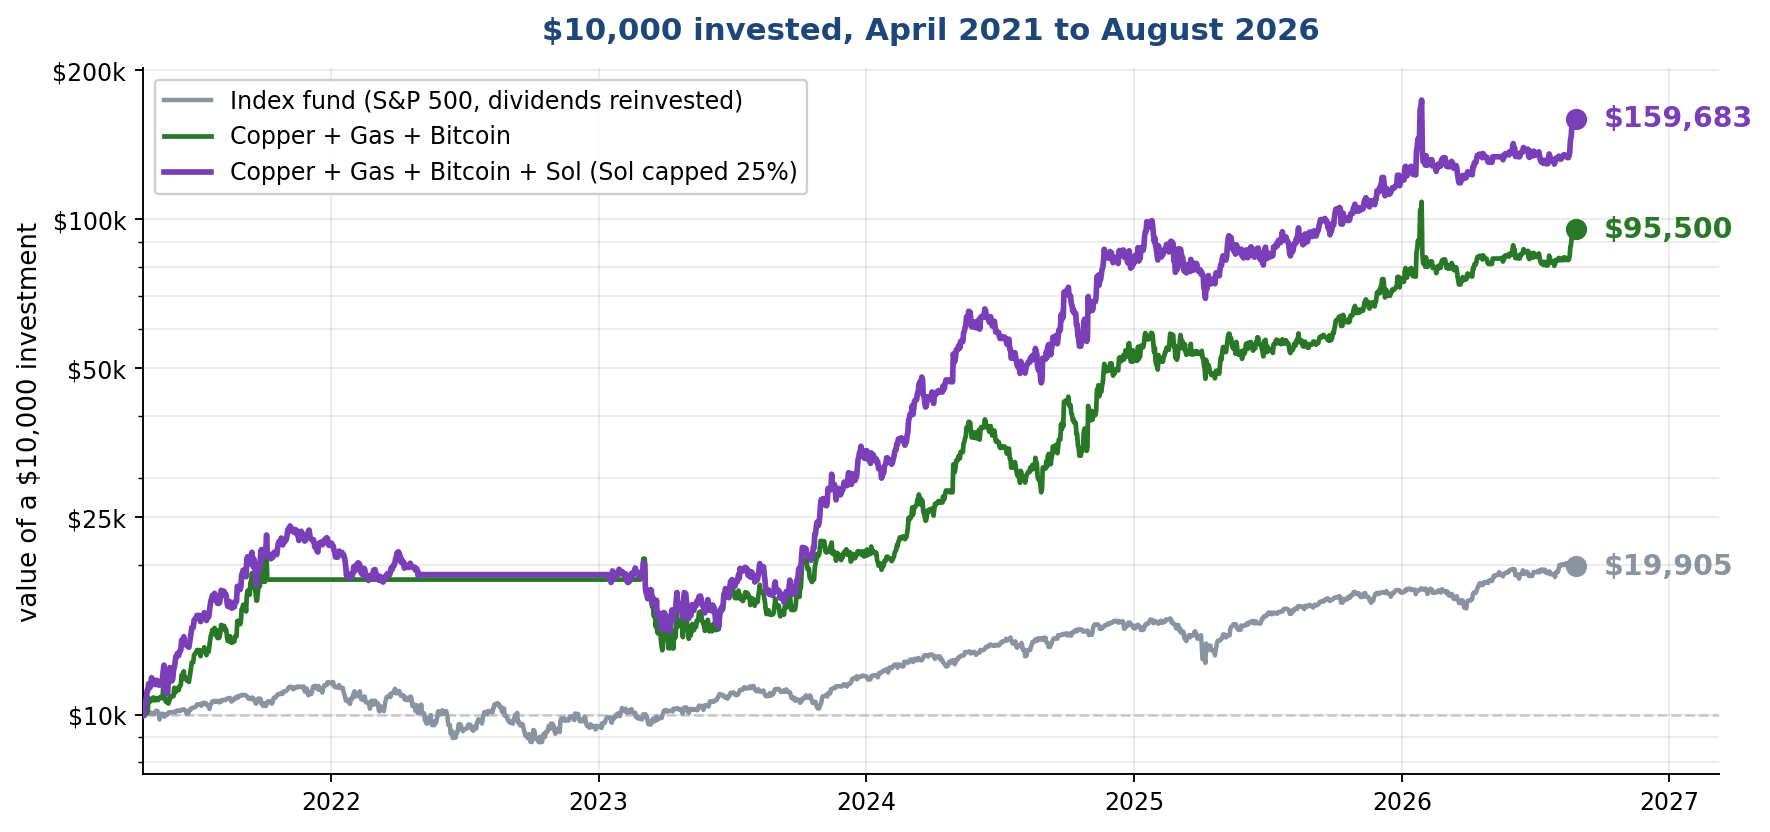
\includegraphics[width=\textwidth]{three_way.png}
\end{figure}

\begin{kbox}[What it adds up to]{strong}
\centering
\begin{tabular}{@{}lrr@{}}
    \toprule
    \textbf{\$10{,}000 in April 2021 became} & & \textbf{Worst drop} \\
    \midrule
    Index fund (S\&P 500)          & \$19{,}905  & $-25\%$ \\
    Copper + Gas + Bitcoin         & \$95{,}500  & $-35\%$ \\
    \textbf{+ Sol, capped at 25\%} & \textbf{\$159{,}683} & \textbf{$-39\%$} \\
    \bottomrule
\end{tabular}

\vspace{0.6em}
\raggedright
\textbf{Notice the long flat stretch in the green line.} That is
\textbf{509 days in a row entirely in cash}, from October 2021 to
February 2023. The rule sat out the whole
2022 crash (COVID). Nothing was
earned --- and nothing was lost.
\end{kbox}

\section{7. The four assets, mildest to wildest}

\begin{kbox}[The risk ladder]{warn}
\centering
\begin{tabular}{@{}llrrr@{}}
    \toprule
    \textbf{Asset} & \textbf{Role} & \textbf{Return} & \textbf{Sharpe} & \textbf{Worst drop} \\
    \midrule
    Copper      & Ballast   & $+97\%$      & $1.05$ & $-23\%$ \\
    Bitcoin     & Flagship  & $+463\%$     & $1.16$ & $-28\%$ \\
    Natural gas & Wildcard  & $+310\%$     & $0.90$ & $-53\%$ \\
    Solana      & Monster   & $+7{,}691\%$ & $1.34$ & $-79\%$ \\
    \bottomrule
\end{tabular}

\end{kbox}

\section{8. Solana: highest risk \emph{and} highest return}

\begin{kbox}[Both things are true, for the same reason]{warn}
\textbf{The best result in the whole study:} $+7{,}691\%$, the highest
Sharpe of anything we tested ($1.34$), wins $18\times$ bigger than its
losses.

\textbf{The most dangerous thing on the list:} a $-79\%$ drop even
\emph{with} the rule. It wins only half its trades. It has the shortest
history.

\vspace{0.6em}
\centering
\textbf{These are not two facts. They are one fact.}

\vspace{0.5em}
\raggedright
The rule makes money from \emph{movement}. A sleepy asset gives it
nothing to work with. Solana's violence is not a side-effect of its
returns --- it is the \emph{source} of them.

\vspace{0.5em}
\begin{center}
\itshape
You cannot have the return of a wild asset\\
without exposure to its wildness.
\end{center}

\end{kbox}

\section{9. Two rules of thumb}

\begin{kbox}[You've got to be in it to win it]{strong}
Cash never lost anyone money, and cash never made anyone any either.

Every number in this document comes from actually being in the market
when the rule says to be. Sitting out entirely is a decision with its
own cost --- you just don't get a statement showing it.

\vspace{0.4em}
The rule is designed so that when you're in, you're in for a reason,
and when you're out, you're out for a reason. Nothing here asks you to
guess.
\end{kbox}

\vspace{0.3em}

\begin{kbox}[But don't bet the farm --- just a portion of it]{warn}
\centering
\Large\bfseries
Only put in money that could go to zero\\
without changing your life.

\vspace{0.6em}
\raggedright\normalsize\normalfont
Starting small is not timidity. It is how you find out whether you can
live with the ride before the ride matters.
\end{kbox}

\vspace{1em}

\newpage
\section{10. Where the rule comes from: a horse race}

\begin{kbox}[The bookmaker does not pick the favourite. You do.]{strong}
Three horses in the Melbourne Cup. Punters have bet \$100{,}000 in
total. The bookmaker didn't decide the odds --- they fall out of
\emph{where the money went}:

\vspace{0.5em}
\centering
\begin{tabular}{@{}lrrr@{}}
    \toprule
    \textbf{Horse} & \textbf{Money on it} & \textbf{Share} & \textbf{Odds} \\
    \midrule
    Thunderbolt  & \$60{,}000 & $60\%$ & $1.67$ to 1 \\
    Silver Arrow & \$30{,}000 & $30\%$ & $3.33$ to 1 \\
    Dark Horse   & \$10{,}000 & $10\%$ & $10$ to 1 \\
    \midrule
    \textbf{Pool} & \textbf{\$100{,}000} & \textbf{$100\%$} & \\
    \bottomrule
\end{tabular}

\vspace{0.6em}
\raggedright
Thunderbolt is the favourite for one reason only: the most money is on
it. The odds are a \textbf{summary of what the crowd believes}, weighted
by how much each believer was willing to risk.
\end{kbox}

\begin{kbox}[Then the money moves --- and so do the odds]{warn}
A rumour goes round that Dark Horse looked extraordinary in a secret
training run. \$20{,}000 of fresh money piles onto it:

\vspace{0.5em}
\centering
\begin{tabular}{@{}lrrr@{}}
    \toprule
    \textbf{Horse} & \textbf{Money on it} & \textbf{Share} & \textbf{Odds} \\
    \midrule
    Thunderbolt  & \$60{,}000 & $50\%$ & $2.0$ to 1 \\
    Silver Arrow & \$30{,}000 & $25\%$ & $4.0$ to 1 \\
    Dark Horse   & \$30{,}000 & $25\%$ & $4.0$ to 1 \\
    \midrule
    \textbf{Pool} & \textbf{\$120{,}000} & \textbf{$100\%$} & \\
    \bottomrule
\end{tabular}

\vspace{0.6em}
\raggedright
Dark Horse has gone from $10$ to 1 down to $4$ to 1. \textbf{Nobody
decided it was faster.} No official reassessed the horse. The horse
didn't change at all.

\vspace{0.4em}
\centering\bfseries
The money moved, so the odds moved.
\end{kbox}

\begin{kbox}[Now swap the horses for Bitcoin]{strong}
A market is the same machine. Every day, people bet:

\vspace{0.4em}
\begin{itemize}[leftmargin=1.6em, topsep=1pt, itemsep=3pt]
    \item \textbf{Buyers} put money into the pool --- they think the
          price should be higher.
    \item \textbf{Sellers} take money out --- they think it should be
          lower.
    \item \textbf{Volume} tells you \emph{how much} money moved.
    \item \textbf{The day's price change} tells you \emph{which way}.
\end{itemize}

\vspace{0.5em}
So a day when Bitcoin rises $3\%$ on heavy trading is a stampede onto
Thunderbolt --- a big, confident bet that the price belongs higher. A
day when it slips $2\%$ on thin trading is a few nervous punters
quietly taking money off the table.

\vspace{0.5em}
\textbf{This is why the rule multiplies the price move by the volume.}
A bet's weight is how much money stood behind it. A $3\%$ move nobody
traded on is a rumour; a $3\%$ move on record volume is a verdict.
\end{kbox}

\begin{kbox}[And that is the whole rule]{strong}
Add up all those daily bets and you get one number --- what \textbf{the
weight of money says the asset is worth}. We call it the
\emph{momentum price}. Compare it to the actual price:

\vspace{0.6em}
\centering
\begin{tabular}{@{}ll@{}}
    \toprule
    \textbf{Pool says \$110k, market says \$95k} & money is flowing
    \emph{in} \\
    & the crowd is backing this horse \\
    & \textcolor{green}{\textbf{$\rightarrow$ hold the asset}} \\
    \midrule
    \textbf{Pool says \$80k, market says \$95k} & money is flowing
    \emph{out} \\
    & the crowd is quietly leaving \\
    & \textcolor{red}{\textbf{$\rightarrow$ hold cash}} \\
    \bottomrule
\end{tabular}

\vspace{0.7em}
\raggedright
\textbf{The strategy is not predicting anything.} It has no opinion on
whether Bitcoin is a good idea, no model of the economy, no forecast.
It only ever asks one question, once a day:

\vspace{0.4em}
\centering\itshape
Is the money still coming in, or has it started leaving?
\end{kbox}

\vspace{1em}

\begin{kbox}[]{warn}
\centering
\large\bfseries Historical returns do not guarantee future returns.

\vspace{0.4em}
\normalsize\normalfont
Everything above is measured on the past. The future has not been
tested. This is research, not advice.
\end{kbox}

\vspace{0.3em}

\enlargethispage{4\baselineskip}
\section*{\normalsize Jargon, if you need it}

{\footnotesize
\setlength{\tabcolsep}{4pt}
\begin{tabular}{@{}lp{11.7cm}@{}}
    \textbf{Alpha}      & Extra return above just buying and holding. The rule's value added. \\
    \textbf{Backtest}   & A simulation over history that already happened. Always flattering. \\
    \textbf{Drawdown}   & The drop from a previous peak. \\
    \textbf{Momentum}   & Trends tend to keep going. The idea the rule rests on. \\
    \textbf{Ratio}      & Our signal. Above 1, hold. Below 1, cash. \\
    \textbf{Sharpe}     & Return per unit of wobble. $1.0$ is good. \\
    \textbf{Volatility} & How much a price jumps around. \\
\end{tabular}
}

\vspace{0.4em}

\begin{kbox}[Not financial advice]{fail}
\color{red}
This document is \textbf{not financial advice}. It is merely a
description of an algorithm which has performed well on historical
data. It is what I \emph{would} do if I had any money.
\textbf{It is not advice for you to do anything with your own.}
\end{kbox}

\end{document}
